\documentclass[12pt,oneside,a4paper]{article}
\usepackage[utf8x]{inputenc}
\usepackage[T1]{fontenc}
\usepackage[english,polish]{babel}
\usepackage{polski}
\usepackage{float}
\usepackage{hyperref} %spis treści niech będzie łączami
\hypersetup{
	plainpages=false,
    colorlinks,
    citecolor=black,
    filecolor=black,
    linkcolor=black,
    urlcolor=black
}
\usepackage{graphicx}
\usepackage{pbox}
\usepackage{tabto}
\usepackage{algorithm}
\usepackage{algpseudocode}
% ustawienia środowiska algorytm
\floatname{algorithm}{Algorytm}
\renewcommand{\algorithmicfunction}{\textbf{funkcja}}
% koniec ustawień

% blokada dzielenia wyrazów (dla kopiowania do Worda)
% \hyphenpenalty 10000
% \exhyphenpenalty 10000
% koniec ustawień blokady

% Rysowanie grafów, schematów, automatów:
\usepackage{pgf}
\usepackage{tikz}
\usetikzlibrary{arrows,automata}

\newtheorem{df}{Definicja}[section]
\newtheorem{concl}[df]{Wniosek}

\begin{document}
\author{Łukasz Marcinkowski}
\author{Łukasz Marcinkowski \and Jacek Sosnowski}
\title{Optymalizacja wydajności wybranych algorytmów grafowych.}
%\pagenumbering{alph}
\maketitle

\section{Testowanie}

\subsection{Wprowadzenie}

Przedmiotem projektu był algorytm odnajdowania cyklu Eulera. 
Jako cel została przyjęta jego implementacja w językach C++ i Java.
Podwójna implementacja miała umożliwić eksperyment polegający na dokładnym zbadaniu wydajności obu podejść.
Ostatecznie w niniejszym sprawozdaniu zostanie uzasadniona odpowiedź na pytania:
\begin{quote}
\textit{
Czy możliwa jest optymalizacja algorytmu poprzez zmianę języka (środowiska) jego implementacji?
A jeśli tak, to jak bardzo znaczącą poprawę można uzyskać?
}
\end{quote}

\subsection{Warunki eksperymentów}

Wstępnie założono, że żadna z implementacji nie zostanie poddana optymalizacji kodu.
Cenniejsze jest uzyskanie czytelnego rozwiązania, aniżeli skomplikowanego i niezrozumiałego kodu.
Jest to sytuacja zbliżona do rzeczywistości -- gdzie zazwyczaj nie ma miejsca na wyścig optymalizacji.

Schemat działania jest wspólny dla obu podejść.
Po pierwsze należy wczytać dane wejściowe (graf) z pliku oraz zbudować odpowiednią strukturę danych w pamięci programu.
Po drugie należy uruchomić implementację algorytmu Fleury'ego (opisanego dokładnie w poprzedniej dokumentacji).


\subsection{Środowisko testowe}

Wszystkie testy były uruchamiane w systemie Ubuntu w wersji 14.04.
Pomiary wydajności zostały wykonane z wykorzystaniem środowiska języka R (za pomocą narzędzia R-Studio).
Znaczenie ma również konfiguracja sprzętowa, która w tym przypadku była oparta na dwurdzeniowym procesorze taktowanym zegarem 2,2 GHz.
Kod źródłowy został skompilowany przez kompilator GCC 4.8 w przypadku języka C++.
Natomiast aplikacja stworzona w Javie podczas testów była uruchamiana z wykorzystaniem platformy JRE w wersji  1.8.

\textbf{Pomiar czasu} był wykonywany z dokładnością do jednej mikrosekundy.
Lecz dla zachowania czytelności niniejszej dokumentacji oraz z uwagi na charakter prowadzonych testów pomiar (czas trwania dłuższy niż sekunda), wyniki są zapisywane z mniejszą precyzją.



\subsection{Testy akceptacyjne}
\label{sub:testy_akceptacyjne}

Zanim oba rozwiązania zostały poddane ocenie wydajności, musiały przejść zestaw testów akceptacyjnych.
Mowa o poszukiwaniu cykli Eulera w prostych grafach wejściowych.
Kilka przykładów przedstawia tabela~\ref{Grafy3TestyAkceptacyjne}.
Więcej grafów znajduje się w katalogach z testami projektu oraz w poprzedniej dokumentacji.

Dla wyjaśnienia, należy zaznaczyć, że ostatni przykład z tabeli \ref{Grafy3TestyAkceptacyjne}
jest tym samym grafem co pierwszy, lecz z dodaną dodatkową krawędzią $(0,3)$.
Taka modyfikacja, sprawiła, że nie można znaleźć cyklu Eulera. 
Istotnie, idąc tą samą drogą, co dla pierwszego grafu, odwiedzone zostaną wszystkie krawędzie oprócz $(0,3)$.
%To pokazuje, że dodanie dowolnej pojedynczej krawędzi do grafu zawierającego cykl Eulera, prowadzi do struktury w której takiego cyklu znaleźć nie można.

Wynikowy cykl Eulera może być zwracany jako tekst przekazany na standardowe wyjście znakowe systemu operacyjnego lub zapisany do pliku.

\begin{table}
\caption{Przykłady grafów stanowiących część testów akceptacyjnych.}
\label{Grafy3TestyAkceptacyjne}
\center

\setlength\tabcolsep{2pt}
\begin{tabular}{l|c|l}

Plik wejściowy & Wygląd grafu & Wynik algorytmu \\
\hline
\hline

\begin{tabular}{l}
directed 5	\\
0 : 1		\\
1 : 4		\\
2 : 3		\\
3 : 4		\\	
4 : 0 2		\\
\end{tabular}
&
\begin{tabular}{l}
% Pięciokąt 5
\begin{tikzpicture}[->,>=stealth',shorten >=1pt,auto,node distance=1.8cm,
                    semithick]
  \tikzstyle{every state}=[fill=red,draw=none,text=white]

  \node[state] 		   (0)                    {$0$};
  \node[state]         (1) [below right of=0] {$1$};
  \node[state]         (2) [below of=1] {$2$};
  \node[state]         (3) [left of=2] {$3$};
  \node[state]         (4) [below left of=0] {$4$};

  \path (0) edge node {} (1)
        (1) edge node {} (4)
        (2) edge node {} (3)
        (3) edge node {} (4)
        (4) edge node {} (0)
        (4) edge node {} (2)
  ; %end path

\end{tikzpicture}
\end{tabular}
&
0, 1, 4, 2, 3, 4, 0
\\
\hline

\begin{tabular}{l}
directed 6	\\
0 : 3		\\
1 : 2		\\
2 : 5		\\
3 : 4		\\
4 : 1		\\
5 : 0		\\
\end{tabular}
&
\begin{tabular}{l}
% Sześciokąt 1
\begin{tikzpicture}[->,>=stealth',shorten >=1pt,auto,node distance=1.8cm,
                    semithick]
  \tikzstyle{every state}=[fill=red,draw=none,text=white]

  \node[state] 		   (0)                    {$0$};
  \node[state]         (1) [right of=0] {$1$};
  \node[state]         (2) [below right of=1] {$2$};
  \node[state]         (3) [below left of=2] {$3$};
  \node[state]         (4) [left of=3] {$4$};
  \node[state]         (5) [below left of=0] {$5$};

  \path (0) edge node {} (3)
        (1) edge node {} (2)
        (2) edge node {} (5)
        (3) edge node {} (4)
        (4) edge node {} (1)
        (5) edge node {} (0)
  ; %end path

\end{tikzpicture}
\end{tabular}
&
3, 4, 1, 2, 5, 0, 3
\\
\hline

\begin{tabular}{l}
directed 5	\\
\textbf{0} : 1 \textbf{3}		\\
1 : 4		\\
2 : 3		\\
3 : 4		\\
4 : 0 2		\\
\end{tabular}
&
\begin{tabular}{l}
% Pięciokąt 5 z krawedzia (0,3)
\begin{tikzpicture}[->,>=stealth',shorten >=1pt,auto,node distance=1.8cm,
                    semithick]
  \tikzstyle{every state}=[fill=red,draw=none,text=white]

  \node[state] 		   (0)                    {$0$};
  \node[state]         (1) [below right of=0] {$1$};
  \node[state]         (2) [below of=1] {$2$};
  \node[state]         (3) [left of=2] {$3$};
  \node[state]         (4) [below left of=0] {$4$};

  \path (0) edge node {} (1)
  		(0) edge node {} (3)
        (1) edge node {} (4)
        (2) edge node {} (3)
        (3) edge node {} (4)
        (4) edge node {} (0)
        (4) edge node {} (2)
  ; %end path

\end{tikzpicture}
\end{tabular}
&
Euler Path: (not found)
\\
\hline
\hline

\end{tabular}

\end{table}




\pagebreak
\section{Porównanie wydajności}

\begin{figure}
\centering
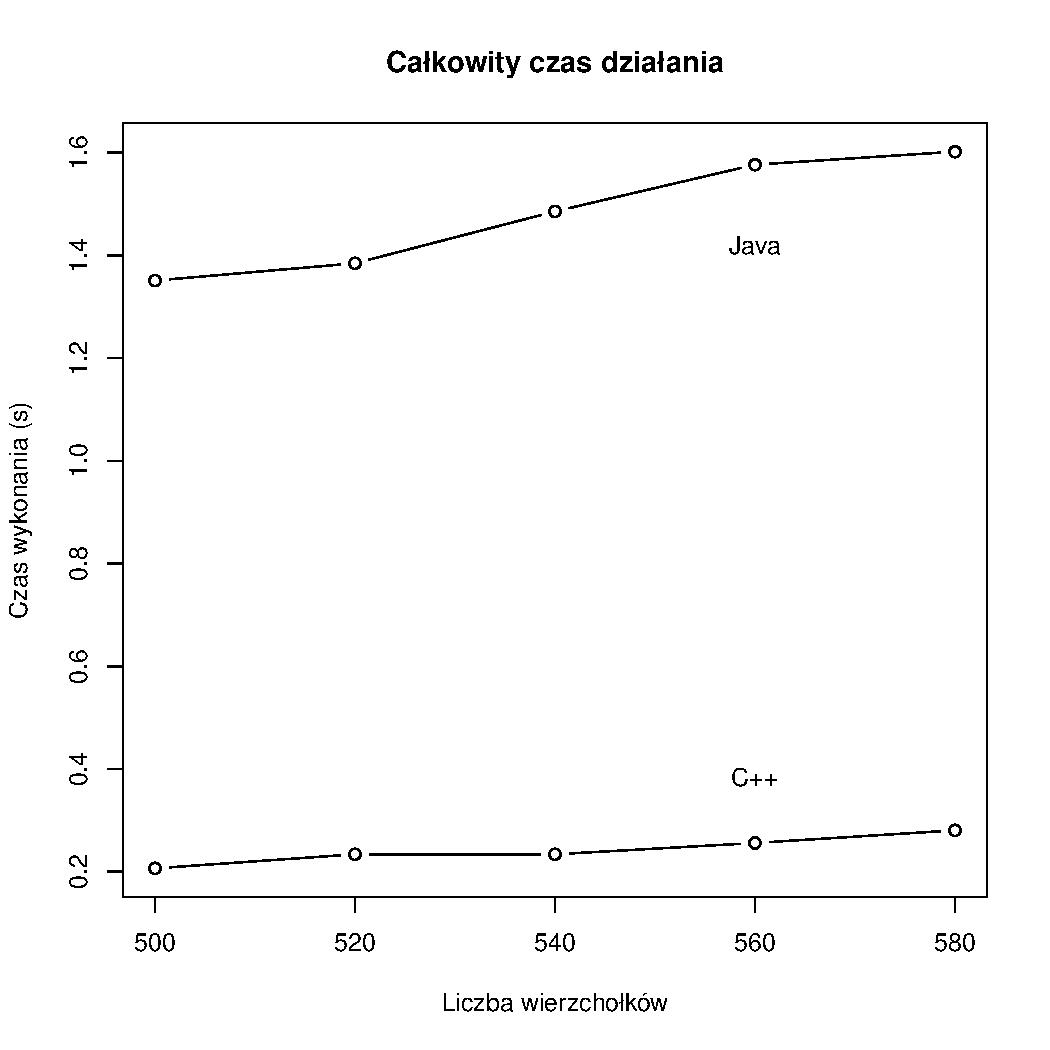
\includegraphics[scale=0.7]{plots/allTimeCompare.pdf}
\caption{Całkowity czas wykonywania zadania.}
\label{p:AllTimeCompare}
\end{figure}

\begin{figure}
\centering
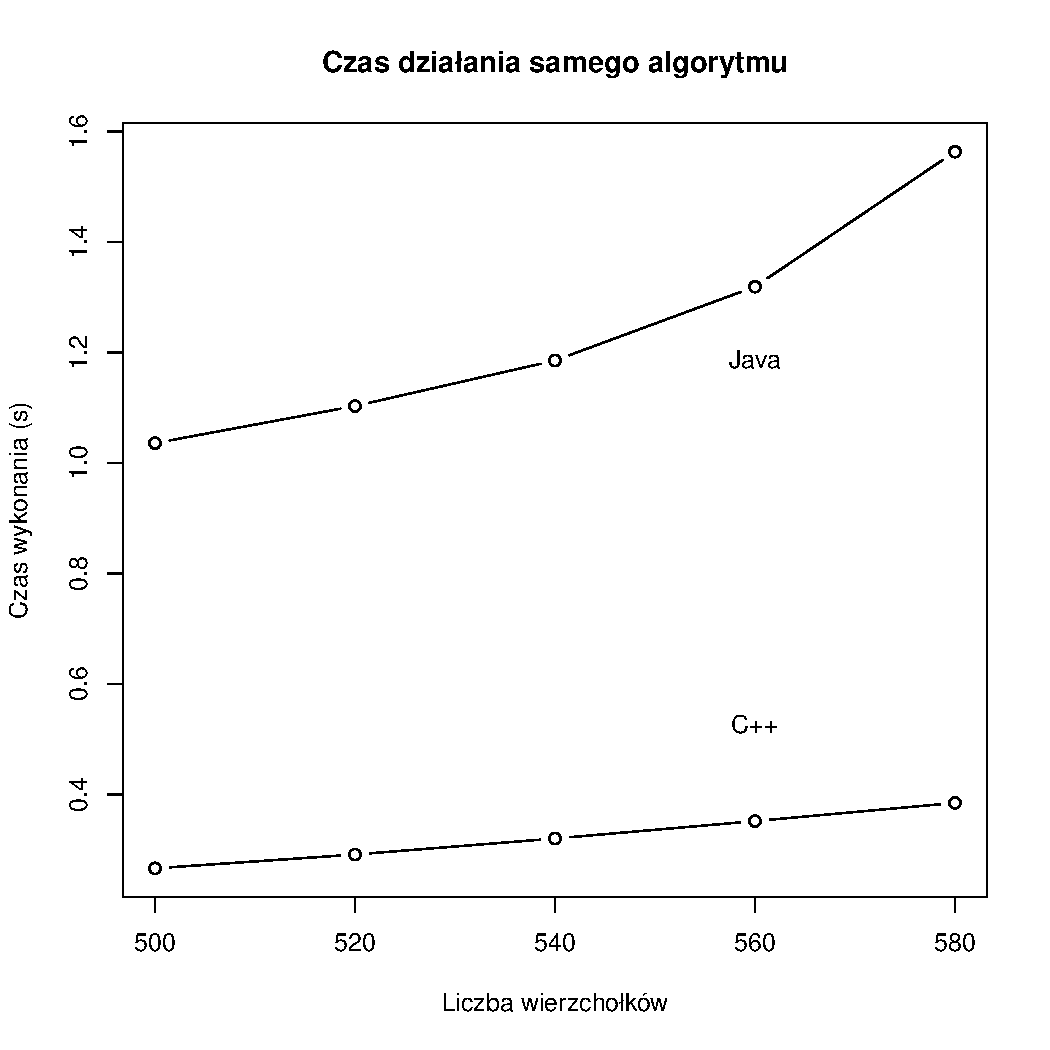
\includegraphics[scale=0.7]{plots/algTimeCompare2.pdf}
\caption{Czas działania algorytmu.}
\label{p:AlgTimeCompare}
\end{figure}

Pierwszy eksperyment reprezentuje wykres \ref{p:AllTimeCompare}.
Nie jest to zbyt sprawiedliwe porównanie, ponieważ pokazuje czas całkowitego uruchomienia (od startu do zwrócenia wyniku).
Z tego powodu, w przypadku implementacji Javy jest również uwzględniany narzut czasowy startu interpretera -- maszyny wirtualnej Javy.

Z tego powodu powstaje pytanie: Czy takie porównanie ma sens? Odpowiedź brzmi: tak, ale wyłącznie z punktu widzenia użytkownika.
Dla niego nie jest istotne w jakiej technologii jest stworzona aplikacja, lecz jak działa.
W tym przypadku widać, że aplikacja Javy zmusza do kilkukrotnie dłuższego oczekiwania na wynik.

Dla usunięcia obciążenia interpretera Javy czas został zmierzony również wewnątrz aplikacji.
Zastosowano rozdzielczość jednej mikrosekundy. 
Wynik przedstawia wykres \ref{p:AlgTimeCompare}.
Jednak jak widać, narzut ten był spory wyłącznie, dla mniejszych danych wejściowych.
Dalej odgrywał już mniejszą rolę.

\subsection{Schemat eksperymentu}

Oba eksperymenty przedstawione na wykresach \ref{p:AllTimeCompare} i \ref{p:AlgTimeCompare}
są wykonane według podobnego schematu:

\begin{enumerate}
\item Generacja (losowanie) grafów o wymaganych własnościach (np. liczbie wierzchołków, krawędzi, itp.)
\item Dla każdego grafu:
	\begin{enumerate}
		\item Kilkukrotne uruchomienie każdej implementacji -- pomiar czasu każdego uruchomienia.
		\item Średnia z powyższych pomiarów jest traktowana jako czas pracy dla określonych danych wejściowych (grafu).	
	\end{enumerate}
\item Tworzenie wykresu.
\end{enumerate}


\subsection{Złożoność}

W paragrafie \ref{sub:testy_akceptacyjne} zostało pokazane, iż aplikacje działają poprawnie.
Jednak należy również zweryfikować złożoność czasową obu rozwiązań.

\begin{figure}
\centering
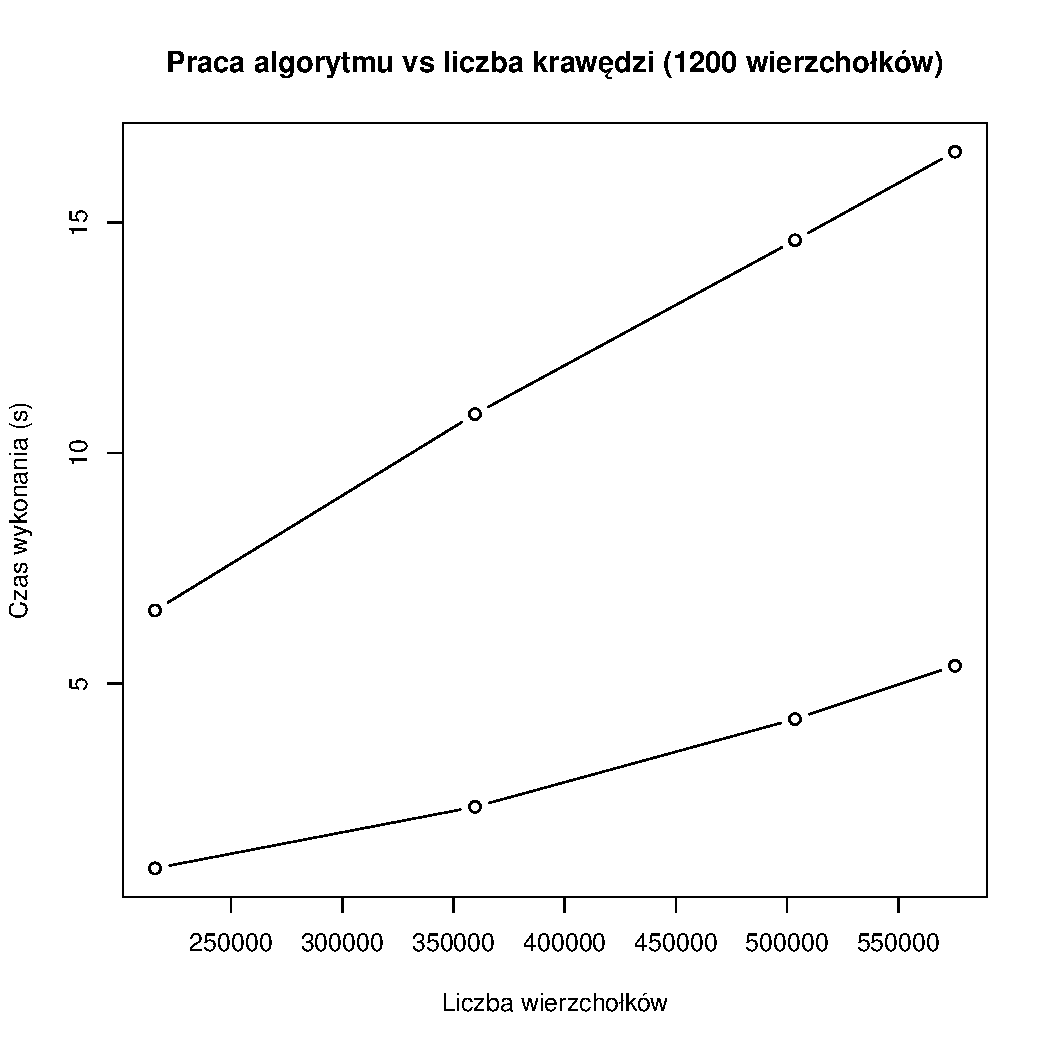
\includegraphics[scale=0.7, trim=0mm 12mm 0mm 0mm, clip]{plots/algTime_vs_edges.pdf}
\caption{Praca algorytmu w zależności do liczby krawędzi. Górny wykres -- Java, dolny -- C++.}
\label{p:AlgTime_vs_edges}
\end{figure}

Jak wskazano w poprzedniej dokumentacji, algorytm Fleury'ego ma złożoność liniową względem liczby krawędzi w grafie. 
W celu weryfikacji tego stwierdzenia, wygenerowano zbiór grafów, każdy o 1200 wierzchołkach ale różnych gęstościach.
Przeliczając gęstość na liczbę krawędzi otrzymano zbiór grafów o licznościach krawędzi pomiędzy 100 tys., a 600 tys.
Wykres \ref{p:AlgTime_vs_edges} pokazuje opisywaną tutaj zależność. 

Jednym z podstawowych wniosków jest fakt, że obie implementacje bezsprzecznie spełniają założenia algorytmu i posiadają złożoność liniową względem liczby krawędzi (O(q), gdzie $q$ to liczba krawędzi).
Ale dodatkowo można zwrócić uwagę na nachylenia obu krzywych.
Okazuje się, że zapotrzebowanie na czas rośnie szybciej w przypadku implementacji w Javie.
Nie jest to wzrost zatrważający, ale może być znaczącym argumentem do zastosowania optymalizacji w postaci zmiany języka z Javy na C++.
Szczególnie wtedy, kiedy wiadomo, że często rozpatrywane będą grafy zbliżone do pełnych.


\subsection{Rozrzut wyników}

Realizując serię pomiarów dla pojedynczej instancji problemu (w tym przypadku -- pojedynczego grafu), należy zauważyć, że każdy pomiar jest realizacją pewnej zmiennej losowej.
Przy porównywaniu obu aplikacji interesujące jest również to jak stabilne są prezentowane wyniki.

\begin{figure}
\centering
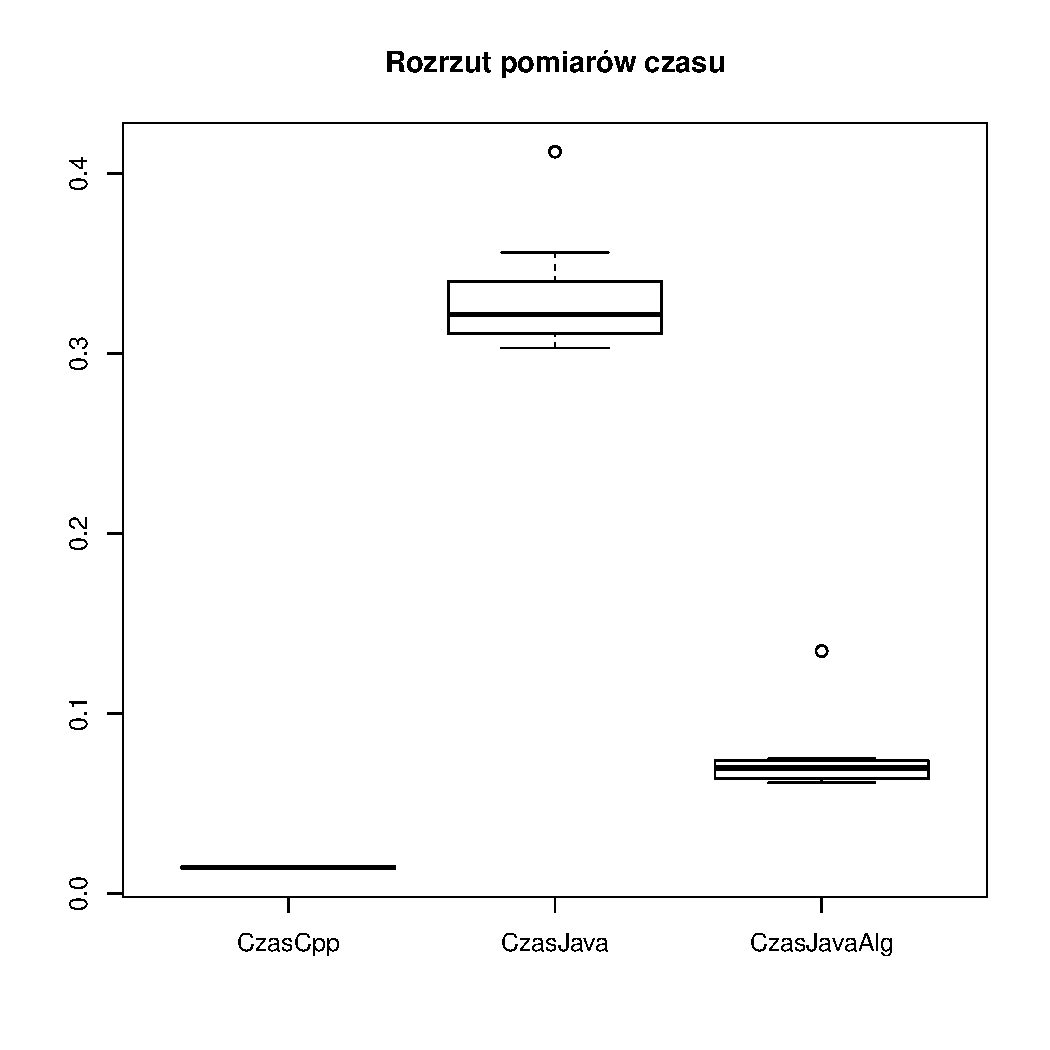
\includegraphics[scale=0.7]{plots/boxPlots.pdf}
\caption{Wykresy pudełkowe: czasu wykonania dla C++, pełnego Javy oraz samego algorytmu w Javie.}
\label{p:BoxPlot}
\end{figure}

Do interpretacji cech statystycznych wykonywanych pomiarów zastosowano wykres pudełkowy (ang. \textit{Box plot}) przedstawiony na Wykresie \ref{p:BoxPlot}.

Największy rozrzut wyników można zaobserwować w przypadku badania pełnego uruchomienia aplikacji w Javie, co może być istotne dla użytkownika końcowego.
Z drugiej strony jest to fakt w pełni uzasadniony działaniem maszyny wirtualnej Javy i systemu operacyjnego.

Dlatego do porównania lepiej zastosować pomiar pracy samego algorytmu, który w tym przypadku pokazuje stabilniejsze działanie. 
Jednak również w tej kategorii niepokonana została implementacja z wykorzystaniem C++. 
Dla której wahania były tak niewielkie, że z racji skali wykresu \ref{p:BoxPlot}, są one niewidoczne.


\subsection{Serie uruchomień}

Na koniec warto przyjrzeć się jeszcze zmienności wyników w perspektywie serii uruchomień każdej z implementacji -- rysunki \ref{p:cppSeries} oraz \ref{p:javaSeries}.

Pokazują one cechę odporności obu implementacji na zmienną gęstość tych samych grafów.
Wyniki są zgodne z oczekiwaniami -- uzyskano zależność liniową -- ale nie jest to cecha oczywista i automatyczna. 
Gdyby w którymś rozwiązaniu zastosowano niewłaściwą strukturę danych (a co za tym idzie nieefektywną), można by zaobserwować znaczące fluktuacje na poszczególnych krzywych.

\begin{figure}
\centering
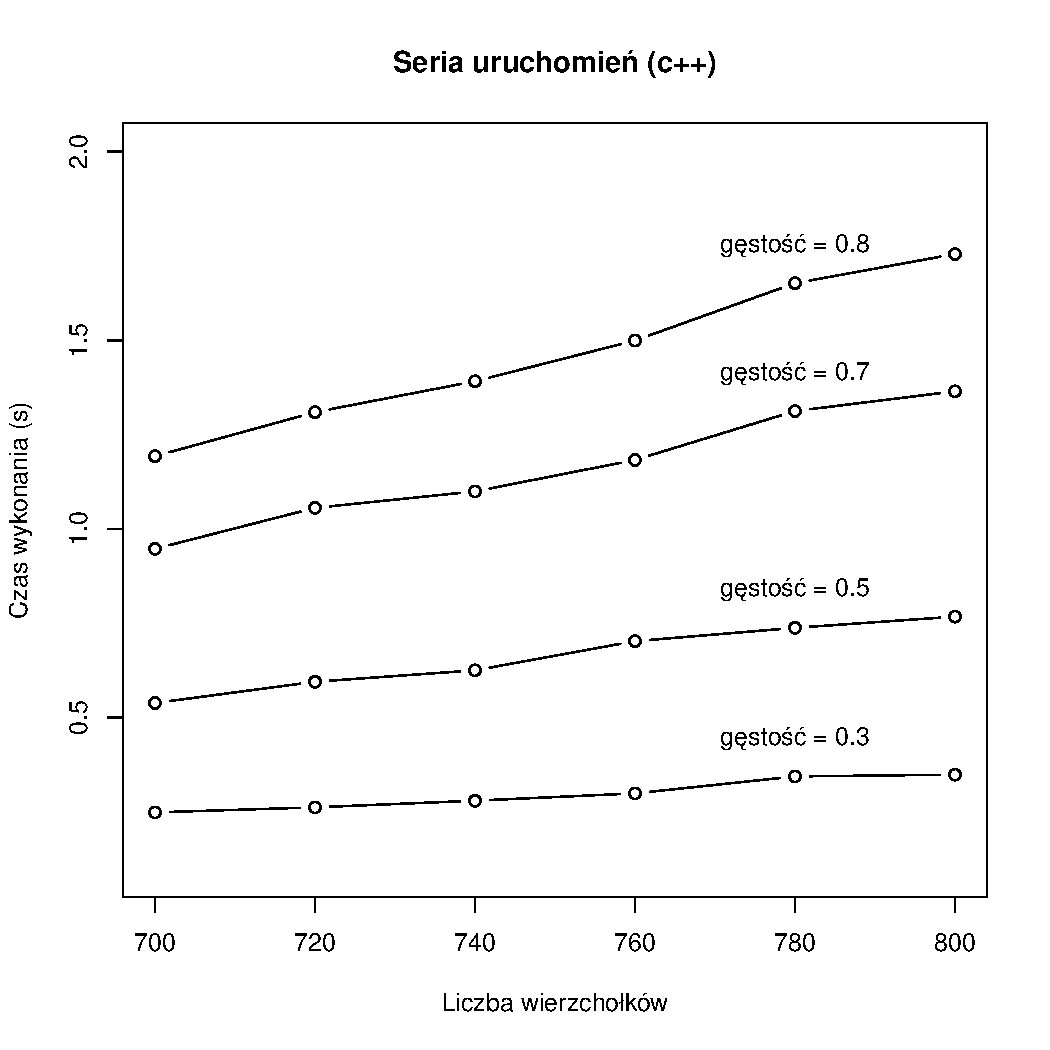
\includegraphics[scale=0.6]{plots/cppTime_inSeries.pdf}
\caption{Seria uruchomień aplikacji napisanej w C++.}
\label{p:cppSeries}
\end{figure}

\begin{figure}
\centering
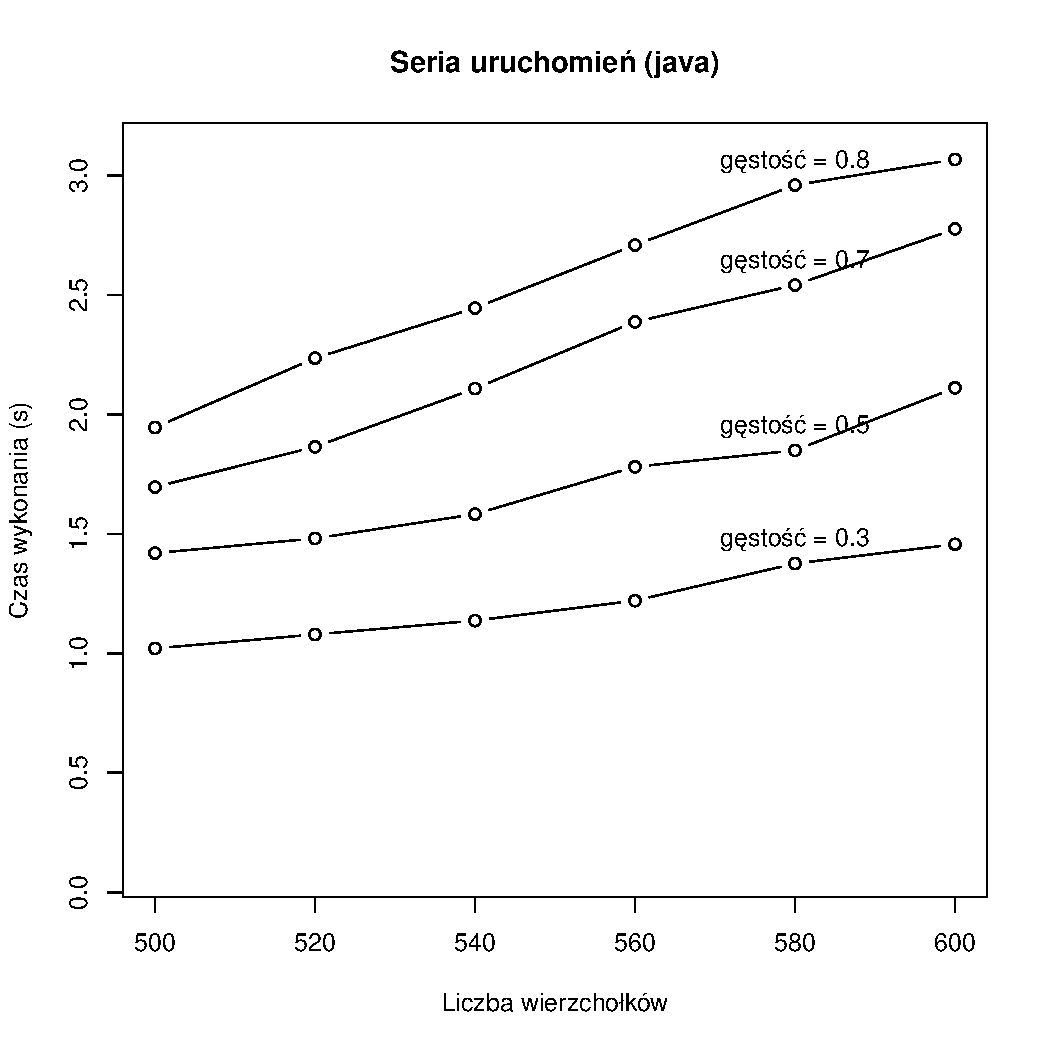
\includegraphics[scale=0.6]{plots/javaTime_inSeries.pdf}
\caption{Seria uruchomień aplikacji napisanej w Javie.}
\label{p:javaSeries}
\end{figure}
\pagebreak
\section{Podsumowanie}

W ramach tego projektu algorytm Fleury'ego został poprawnie zaimplementowany w dwóch najbardziej popularnych językach obecnego świata IT.
Przeprowadzono szereg różnorodnych wyszukiwań cykli Eulera na losowych grafach o różnych liczbach wierzchołków i krawędzi.
Testowano grafy od najmniejszego trój-wierzchołkowego, po takie o liczbie wierzchołków rzędu tysięcy.
Ponadto dokonano wielu badań, których wyniki zostały zaprezentowane w niniejszym sprawozdaniu.

Na podstawie zdobytych doświadczeń, a także w ramach podsumowania można wysnuć wniosek o istnieniu \textbf{optymalizacji} w kontekście zmiany języka implementacji dla algorytmów grafowych.
Innymi słowy, pokazano tutaj, że ten sam algorytm osiąga znacząco różne rezultaty w różnych językach.
Nie zakłada się, że cechą obu języków jest fakt, że jeden jest efektywniejszy od drugiego.
Ale posiadając kod Javy implementujący pewien algorytm grafowy (np. poszukujący cykli Eulera) jest wielce prawdopodobne, że jego ,,przepisanie'' w języku C++ przyniesie korzyść w postaci zmniejszonej konsumpcji czasu.
Jest to w rzeczywistości pewien rodzaj optymalizacji, który można osiągnąć stosunkowo niskim kosztem oraz bez ryzyka straty czytelności samego kodu źródłowego.



\pagebreak
%%%%%
%% Bibliografia

\begin{thebibliography}{9}

\bibitem{Wojciechowski} J. Wojciechowski, K. Pieńkosz, \emph{Grafy i sieci}, Wydawnictwo Naukowe PWN, 2013

\bibitem{Cormen} T.H. Cormen, C.E. Leiserson, R.L. Rivest, \emph{Wprowadzenie do algorytmów}, Wydawnictwo
Naukowo-Techniczne, Warszawa 2001.

\end{thebibliography}

\end{document}